\documentclass[12pt]{article}
%\usepackage{xcolor}
\usepackage[top=2cm, bottom=2cm, left=2cm, right=2cm, headsep=2mm, foot=4mm]{geometry}
\usepackage{amsmath,amsthm,amsfonts,amssymb,amscd}
\usepackage{enumitem}
\usepackage{parskip}
\usepackage{mathtools}
\usepackage{mathrsfs}
\usepackage{mdframed}
\usepackage{fancyhdr}
\usepackage{graphicx}
\usepackage{hyperref}
\graphicspath{ {./img/} }
\usepackage{float}
\usepackage{caption}
\usepackage{subcaption}

\pagestyle{fancy}
\title{Homework 2 - AMATH 563}
\author{Warren Paris-Moe}
\date{April 2023}
\fancyhf{}
\fancyhead[C]{{\small \emph{W. Paris-Moe / Homework 2 Writeup | AMATH 563}}}
\fancyhead[R]{\emph{\thepage}}
\renewcommand{\headrulewidth}{0.4pt}
\renewcommand{\footrulewidth}{0.4pt}

\newcommand\tk{\tilde k}\newcommand\ip[2]{\langle #1,#2\rangle}

\begin{document}
\maketitle

\section*{THEORY}

\subsection*{Problem 1}
\begin{mdframed}
    Suppose $\Gamma: \mathcal{X} \times \mathcal{X} \to \mathbb{R}$ is a PDS kernel. 
    Prove that $\forall x, x' \in \mathcal{X}$ it holds that
    $|\Gamma(x, x')|^2 \leq \Gamma(x, x) \Gamma(x', x')$.
\end{mdframed}

Let $\Gamma:\mathcal{X}\times\mathcal{X}arrow\mathbb{R}$ be a positive definite symmetric (PDS)
kernel in the real space and $x,x' \in \mathcal{X}$. Say $x=x_1$ and $x'=x_2$. Then, since $\Gamma$ 
is PDS, we know that the $2 \times 2$ kernel matrix $K$ with entries $K_{ij} = \Gamma(x_i, x_j)$ is 
positive definite. Therefore, its eigenvalues are nonnegative. Thus, it follows that the product of 
those eigenvalues, aka the determinant of $K$, is also nonnegative. That is,
\begin{align*}
    0 \leq K_{11}K_{22} - K_{12}K_{21} &= K_{11}K_{22} - K_{12}K_{12}^* \\
    &= K_{11}K_{22} - |K_{12}|^2 \\
    &= \Gamma(x_1, x_1)\Gamma(x_2, x_2) - |\Gamma(x_1, x_2)|^2 \\
    &= \Gamma(x, x)\Gamma(x', x') - |\Gamma(x, x')|^2
\end{align*}
where $K_{12}^*$ is the complex conjugate of $K_{12}$. Since $\Gamma$ is real-valued,
$K_{12}^* = K_{12}$. Thus, we have that 
\begin{align}
    |\Gamma(x, x')|^2 \leq \Gamma(x, x)\Gamma(x', x')
\end{align}


\subsection*{Problem 2} % Problem 2
\begin{mdframed}
    Given a kernel $K$ on $\mathcal{X}$ define its normalized version as
    \[
    \bar{K}(x,x') = 
        \begin{cases}
            0 & \text{if } K(x,x)=0 \text{ or } K(x', x')=0 \\ 
            \frac{K(x, x')}{\sqrt{K(x, x)} \sqrt{K(x', x')}} & \text{Otherwise.} 
        \end{cases}
    \]
    Show that if $K$ is PDS then so is $\bar{K}$.
\end{mdframed}

Notice when $K(x, x) = 0$ or $K(x', x') = 0$, we see that $\bar{K}(x, x') = 0$ so it the
normalized kernel is positive definite. Now, examining the else case for positive definiteness and
using the feature map representation of $K$, we have that for $c_1, c_2, \dots, c_n \in \mathbb{R}$,
\begin{align*}
    \sum_{i,j=1}c_ic_j\hat{K}(x_i,x_j) &= \sum_{i,j=1}\frac{c_ic_jK(x_i, x_j)}{\sqrt{K(x_i, x_i)} \sqrt{K(x_j, x_j)}} \\
    &=\sum_{i,j=1}\frac{c_ic_j\langle\varphi_{x_i},\varphi_{x_j}\rangle}{\sqrt{\langle\varphi_{x_i},\varphi_{x_i}\rangle}\sqrt{\langle\varphi_{x_j},\varphi_{x_j}\rangle}} \\
    &=\sum_{i,j}\frac{c_ic_j\langle\varphi_{x_i},\varphi_{x_j}\rangle}{\sqrt{\|\varphi_{x_i}\|^2}\sqrt{\|\varphi_{x_j}\|^2}} \\
    &=\sum_{i,j=1}\frac{c_ic_j\langle\varphi_{x_i},\varphi_{x_j}\rangle}{\|\varphi_{x_i}\| \|\varphi_{x_j}\|} \\
    &=\sum_{i=1}\|\frac{c_i\varphi_{x_i}}{\|\varphi_{x_i}\|}\|^2 \\
    &\geq 0
\end{align*}
since $K$ is PDS. We can see that the symmetry of the normalized kernel $\hat{K}(x,x')=\hat{K(x',x)}$ is trivial. 
Thus, we have that $\bar{K}$ is PDS.

Note: The goal of using the normalized kernel is to ensure that points in the feature space have unit length, or norm.
This process is, in effect, equivalent to replacing $\varphi(x_i)$ with $\frac{\varphi(x_i)}{\|\varphi(x_i)\|}$.


\subsection*{Problem 3} % Problem 3
\begin{mdframed}
    Show that the following kernels on $\mathbb{R}^{d}$ are PDS:
    \begin{itemize}
        \item Polynomial kernel: $K(x, x')=(x^{T} x'+c)^{\alpha}$ for $c>0$ and $\alpha \in \mathbb{N}$.
        \item Exponential kernel: $K(x, x')=\exp (x^Tx')$.
        \item RBF kernel: $K(x, x')=\exp (-\gamma^{2}\|x-x'\|_2^2)$.
    \end{itemize}
\end{mdframed}

\subsubsection*{Polynomial Kernel}
Let $K(x, x') = (x^Tx' + c)^\alpha$ for $c > 0$ and $\alpha \in \mathbb{N}$. Then, we have that
\begin{align*}
    K(x, x') = (x^Tx' + c)^\alpha = (x'^Tx + c)^\alpha = K(x', x)
\end{align*}
showing that the kernel is symmetric. Now, if we expand out the expression into a sum with 
non-negative coefficients, the result is a sum of of positive definite kernels $\langle x,x'\rangle=x^Tx'$
raised to integer powers. Each individual term is a valid kernel by the the product rule of kernels.
By using the binomial formula we can see that the polynomial kernel is PDS since it is a sum of PDS kernels:
\begin{align*}
    K(x, x') = (x^T x' + c)^\alpha = \sum_{k=1}^\alpha \binom{\alpha}{k} c^{\alpha - k}(x^Tx')^k
\end{align*}

\subsubsection*{Exponential Kernel}
Let $K(x, x') = \exp(x^Tx')$. Then, using the taylor approximation of the exponential function
\[
    \exp{(x)} = \lim_{k \to \infty} (\sum_{i=0}^k \frac{x^i}{i!})  = \lim_{k \to \infty} (1 + x + \dots + \frac{x^k}{k!})
\]
we have 
\[
    K(x,x') = \exp{(x^Tx')} = \lim_{k \to \infty} (1 + (x^Tx') + \dots + \frac{(x^Tx')^k}{k!})
\]
where we can see that the exponential kernel is just a sum of PDS kernels $\langle x,x'\rangle=x^Tx'$
raised to degree $i$, multiplied by non-negative coefficients. Thus, by the sum and product rules of 
kernels, the exponential kernel is PDS.


\subsubsection*{RBF Kernel}
By applying the taylor expansion of the exponential function and some reworking of the Gaussian kernel,
we can show that it is PDF. First, using the fact that $\|x-x'\|^2 = \|x\|^2 + \|x'\|^2 - 2x^Tx'$, 
we rewrite the RBF kernel as
\begin{align*}
    K(x,x') &= \exp(-\gamma^2\|x-x'\|_2^2) \\
    &= \exp{(-\gamma^2 \|x\|^2)} \exp{(-\gamma^2 \|x'\|^2)} \exp{(2\gamma^2 x^Tx')} \\ 
    &= f(x)f(x')\exp{(2\gamma^2 x^Tx')}
\end{align*}
where $f(x)=\exp{(-\gamma^2 \|x\|^2)}$ is a positive function. By the tensor product rule of kernels, more specifically a 
conformal transformation, we have that $f(x)f(x')$ is a PDS kernel.
Applying the infinite talor expansion to the last term, we get
\begin{align*}
    \exp{(2\gamma^2 x^Tx')} &= \sum_{k=0}^\infty \frac{(2\gamma^2 x^Tx')^k}{k!} \\
    &= \sum_{k=0}^\infty \frac{(2\gamma^2)^k}{k!}(x^Tx')^k \\
    &= 1 + (2\gamma^2) x^Tx' + \frac{(2\gamma^2)^2}{2}(x^Tx')^2 + \frac{(2\gamma^2)^3}{6}(x^Tx')^3 + \dots
\end{align*}
which following logic similar to the exponential kernel, we can see that $\exp{(2\gamma^2 x^Tx')}$ is PDS,
and thus the RBF kernel is PDS as it is the product of two valid PDS kernels.


\subsection*{Problem 4} % Problem 4
\begin{mdframed}
    Let $\Omega \subseteq \mathbb{R}^{d}$ and let $\{\psi_j\}_{j=1}^n$ be a sequence of continuous 
    functions on $\Omega$ and $\{\lambda_j\}_{j=1}^n$ a sequence of non-negative numbers. Show that 
    $K(x,x')=\sum_{j=1}^n \lambda_j\psi_j(x)\psi_j(x')$ is a PDS kernel on $\Omega$.
\end{mdframed}
Let $c \in \mathbb{R}^m$ be an arbitrary vector of constants. Then, we have that
\begin{align*}
    \sum_{i,j=1}^m c_i c_j K(x_i, x_j) &= \sum_{i,j=1}^m c_i c_j \sum_{k=1}^n \lambda_k \psi_k(x_i)\psi_k(x_j) \\
    &= \sum_{k=1}^n \lambda_k \sum_{i,j=1}^m c_i c_j \psi_k(x_i)\psi_k(x_j) \\
    &= \sum_{k=1}^n \lambda_k \left(\sum_{i=1}^m c_i \psi_k(x_i)\right)^2 \geq 0
\end{align*}
where the last inequality follows from the fact that the square of a real number is non-negative and
the sequence $\{\lambda_j\}_{j=1}^n$ is non-negative. Thus, we have that 
$K(x,x')=\sum_{j=1}^n \lambda_j\psi_j(x)\psi_j(x')$ is a PDS kernel on $\Omega$.


\subsection*{Problem 5} % Problem 5
\begin{mdframed}
    Show that:
    \begin{enumerate}[topsep=0pt, partopsep=0pt, itemsep=0pt, label=(\roman*)]
        \item if $K$ and $K'$ are two reproducing kernels for an RKHS $\mathcal{H}$, 
            then they have to be the same. \\
        \item the RKHS of a PDS kernel $K$ is unique.
    \end{enumerate}
\end{mdframed}

\begin{enumerate}[topsep=0pt, partopsep=0pt, itemsep=0pt, label=(\roman*)]
    \item Suppose that $K$ is a reproducing kernels for an RKHS $\mathcal{H}$ on a set $X$. 
        Let $x,x'\in X$ and $f\in \mathcal{H}$. Since $K$ is a reproducing kernel, we have that 
        $f(x)=\langle f, K_x\rangle$ and $K(x,x') = \langle K_x, K_{x'}\rangle = K_x(x')$ where 
        $\langle \cdot,\cdot\rangle$ is an inner product on $\mathcal{H}$. 
        Similarly, let $K'$ be another reproducing kernel for $\mathcal{H}$ on $X$ with identical 
        properties. Then, $\forall x \in X$, we have that
        \begin{align*}
            \|K_x - K'_x\|^2 &= \ip{K_x - K'_x}{K_x - K'_x} \\
            &= \ip{K_x}{K_x}+\ip{K'_x}{K'_x}-\ip{K_x}{K'_x}-\ip{K'_x}{K_x} \\ 
            &= K(x,x)+K'(x,x)-K_x(x)-K'_x(x) \\
            &= K(x,x)+K'(x,x)-K(x,x)-K'(x,x) \\
            &=0
        \end{align*}
        Therefore, we have that $K_x = K'_x$ for all $x \in X$, and thus $K=K'$.

    \item Suppose that $K$ is a PDS kernel on a set $X$ so that $\forall x \in X, K_x = K(x, \cdot)$.
        Now, let $\mathcal{H}_0$ be the linear span of $\{K_x\}_{x\in X}$. Then, we define an inner 
        product on $\mathcal{H}_0$ as follows:
        \[
            \ip{\sum_{j=1}^n b_j K_{x_j}}{\sum_{i=1}^m a_i K_{x'_i}} = \sum_{i,j=1}^{m,n} a_i b_j K(x_j, x'_i)
        \]
        where $a_i, b_j \in \mathbb{R}$ and $x, x' \in X$. The above implies that $K(x,x')=\ip{K_x}{K_{x'}}_{\mathcal{H}_0}$.
        Notice that since $K$ is symmetric, the inner product must also be symmetric, ie:
        $\ip{K_x}{K_{x'}}_{\mathcal{H}_0} = \ip{K_{x'}}{K_x}_{\mathcal{H}_0}$. \\
        Let $\mathcal{H}$ be the completion of $\mathcal{H}_0$ equipped with the inner product defined above.
        Then, $\mathcal{H}$ is made up of functions of the form
        \[
            f(x) = \sum_{i=1}^{\infty} a_i K_{x_i}(x)
        \]
        where 
        \[
            \lim_{n\to \infty} \sup_{p\geq 0} \| \sum_{i=n}^{n+p} a_i K_{x_i} \|_{\mathcal{H}_0} = 0.
        \] 
        Next, we check for the reproducing property
        \[
            \ip{f}{K_x}_{\mathcal{H}} = \sum_{i=1}^{\infty} a_i \ip{K_{x_i}}{K_x}_{\mathcal{H}_0} = \sum_{i=1}^{\infty} a_i K(x_i, x) = f(x)
        \]
        Now, let $\mathcal{H}'$ be another RKHS of $K$ on $X$. Then, $\forall x,x' \in X$, we have that
        \[
            \ip{K_x}{K_{x'}}_{\mathcal{H}_0} = K(x,x') = \ip{K_x}{K_{x'}}_{\mathcal{H}'}.
        \]
        We can observe that the inner products on $\mathcal{H}_0$ and $\mathcal{H}'$ are identical by linearity
        on the span of $\{K_x : x\in X\}$, $\ip{\cdot}{\cdot}_\mathcal{H} = \ip{\cdot}{\cdot}_{\mathcal{H}'}$.
        It follows that $\mathcal{H} \subset \mathcal{H}'$ since $\mathcal{H}'$ is complete and contains
        $\mathcal{H}_0$ meaning it must contain its completion as well. \\
        Furthermore, let $f$ be an element of $\mathcal{H}'$. Then, as $\mathcal{H}$ is a closed subspace of $\mathcal{H}'$,
        we have that $f = f_{\mathcal{H}} + f_{\mathcal{H}^\perp}$ where $f_{\mathcal{H}} \in \mathcal{H}$ and
        $f_{\mathcal{H}^\perp} \in \mathcal{H}^\perp$. Here, $\mathcal{H}^\perp$ is the orthogonal complement to $\mathcal{H}$.
        Then, we have that for any $x \in X$, following from the fact that $K$ is a reproducing kernel for both $\mathcal{H}'$
        and $\mathcal{H}$,
        \begin{align*}
            f(x) &= \ip{K_x}{f}_{\mathcal{H}'} \\
            &= \ip{K_x}{f_{\mathcal{H}}}_{\mathcal{H}'} + \ip{K_x}{f_{\mathcal{H}^\perp}}_{\mathcal{H}'} \\
            &= \ip{K_x}{f_{\mathcal{H}}}_{\mathcal{H}'} \\
            &= \ip{K_x}{f_{\mathcal{H}}}_{\mathcal{H}} \\
            &= f_{\mathcal{H}}(x).
        \end{align*}
        The above derivation comes from the idea that $K_x$ belongs to $\mathcal{H}$ meaning that it is orthogonal to
        $f_{\mathcal{H}^\perp}$ in $\mathcal{H}'$ (ie: its inner product with $f_{\mathcal{H}^\perp}$ in $\mathcal{H}'$ is zero).
        This implies that every element of $\mathcal{H}'$ is also an element of $\mathcal{H}$, and thus 
        $\mathcal{H}' \subset \mathcal{H}$ so that $f=f_\mathcal{H}$ in $\mathcal{H}'$. Therefore, we can conclude that
        if $K$ is a PDS kernel on $X$, then $\mathcal{H}$ is the unique RKHS of $K$ on $X$.


\end{enumerate}
\newpage

\section*{COMPUTATION}

\subsection*{MNIST DATASET}
% Explain the dataset
The MNIST dataset is a collection of 70,000 images of handwritten digits. Each image is a 28x28 pixel image  that is 
projected into a 784 dimensional vector. Each pixel is represented by a value between 0 and 255, where 0 is white and 255 is black.
The dataset is split into 60,000 training images and 10,000 test images. \\
% include figure `mnist-digits.png`
\begin{figure}[h!]
    \centering
    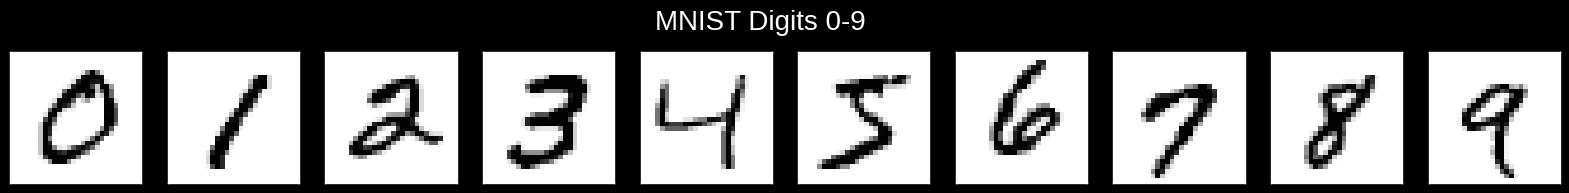
\includegraphics[scale=0.4]{mnist-digits.png}
\caption{MNIST digits}
\label{fig:mnist}
\end{figure}

Digits 0-9 of the MNIST dataset are shown in Figure \ref{fig:mnist}. One issue with the dataset is that the images are not centered
making it more difficult for a classifier to learn the features of the digits. Also, since the images are supposed to be of handwritten
digits, there is a lot of variation in the way the digits are written. For example, the digit 4 can be written with a straight line or
with a curved line. This makes it even more difficult for a classifier to learn the features of the digits. Variation within the dataset
among the digit 1 is shown in Figure \ref{fig:ones}, and variation among the digit 7 in Figure \ref{fig:sevens}. \\
% include figure `ones.png`
\begin{figure}[htbp]
    \centering
    \begin{subfigure}[b]{0.45\textwidth}
        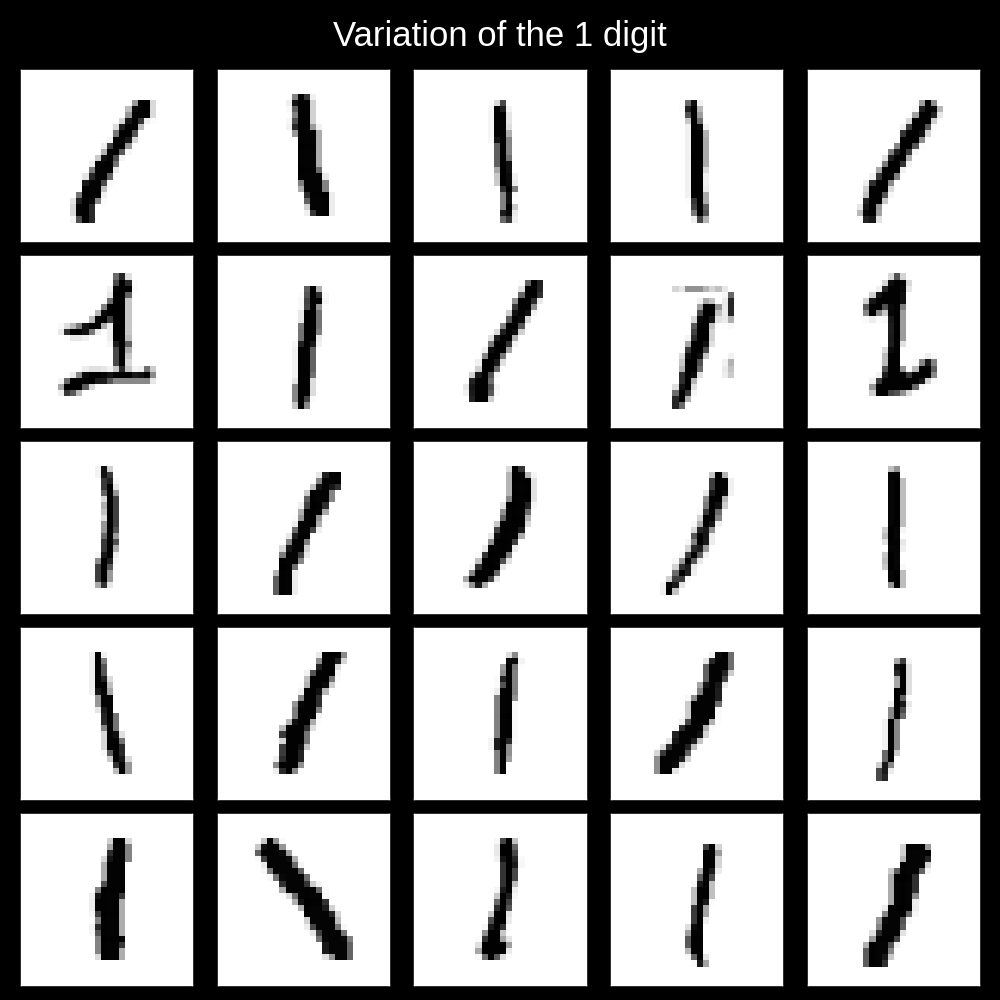
\includegraphics[width=\textwidth]{ones.png}
        \caption{Variation in the digit 1.}
        \label{fig:ones}
    \end{subfigure}
    \hfill
    \begin{subfigure}[b]{0.45\textwidth}
        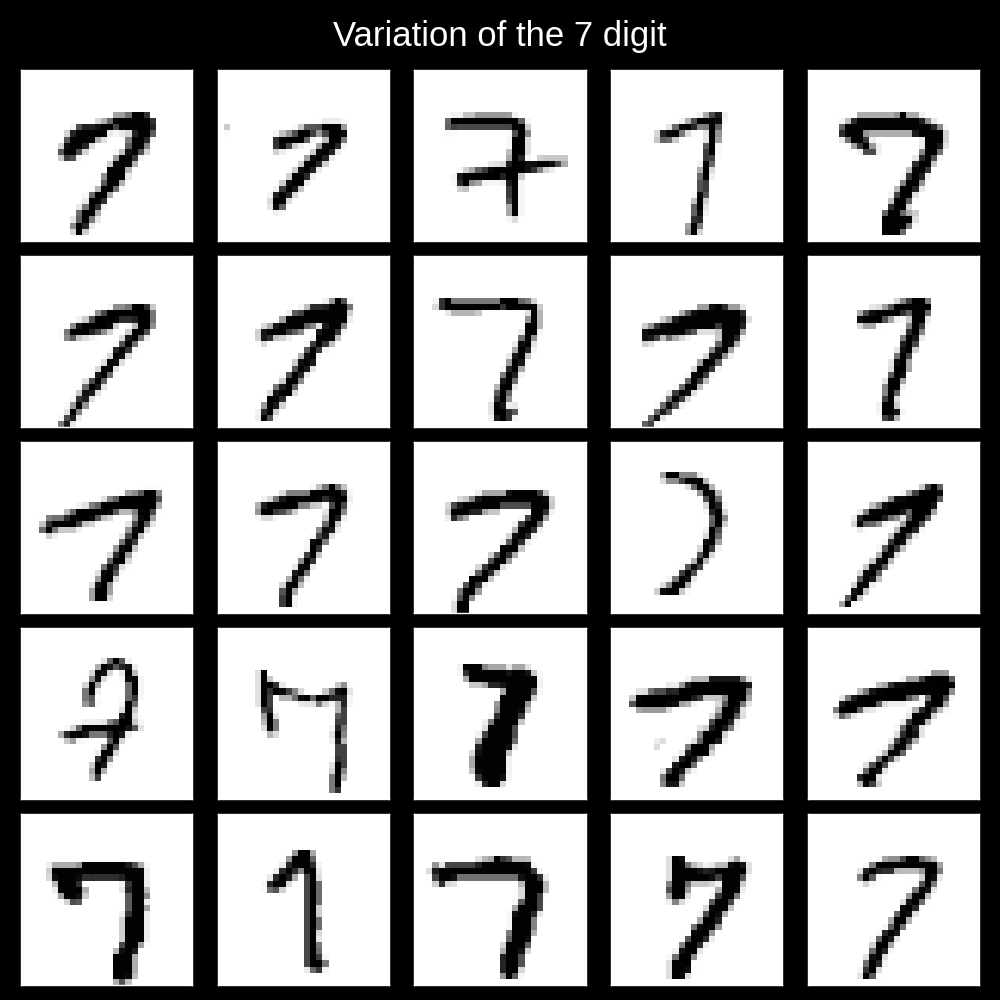
\includegraphics[width=\textwidth]{sevens.png}
        \caption{Variation in the digit 7.}
        \label{fig:sevens}
    \end{subfigure}
    \caption{Variation in the MNIST dataset.}
    \label{fig:variation}
\end{figure}

\subsection*{PREPROCESSING}
% Explain the preprocessing steps (PCA)
Principal component analysis (PCA) was used to reduce the dimensionality of the dataset. 
PCA was implemnted using an eigendecomposition method. We define 
$\boldsymbol{\mathbf{\Sigma}}$, a $784 \times 784$ matrix, as follows: 
\[
\boldsymbol{\mathbf{\Sigma}} = \frac{1}{n} \sum_{i=1}^n \boldsymbol{\mathbf{x}}_i {\boldsymbol{\mathbf{x}}}^{\mathrm{T}}_i
\]
where the $\boldsymbol{\mathbf{x}}_i$’s are points in our dataset as column vectors and $n = 60,000$ is the number 
of points in the training dataset. Now compute the top $k$ PCA dimensions; these are the $k$ dimensions which best 
reconstruct the data. The top $k$ PCA dimensions (modes) are the eigenvectors corresponding to the $k$ largest eigenvalues.
The eigenvalues were sorted in descending order and the top $k$ eigenvectors were selected based on maximizing the
the total sum of the eigenvalues (ie: the top $k$ eigenvectors were selected such that they preserved 95\% of the variance).
The top 95\% of the variance was preserved by selecting the top 154 eigenvectors. The dataset was then projected onto
the top 154 eigenvectors to reduce the dimensionality of the dataset. \\

% Plot the PCA modes for k=154
\begin{figure}[h!]
    \centering
    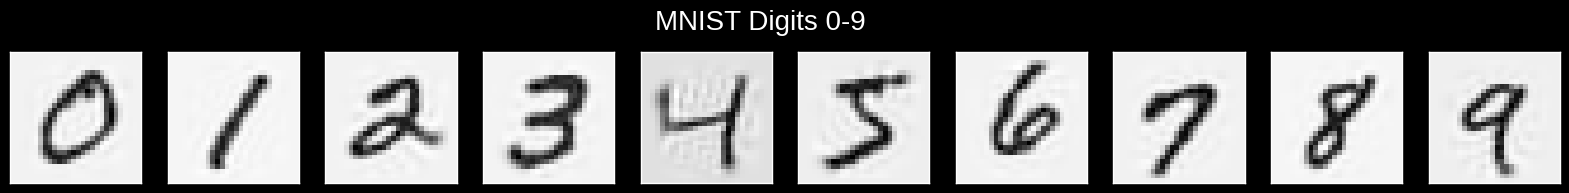
\includegraphics[scale=0.4]{mnist_pca.png}    
    \caption{PCA modes for $k=154$.}
    \label{fig:pca}
\end{figure}

Figure \ref{fig:pca} shows the same images as Figure \ref{fig:mnist} reconstructed using the top 154 PCA modes. 
As we can see from the figure, the images are still recognizable after being projected onto the top 154 PCA modes.
Some of the digits are not as clear as the original images, but the general structure of the digits is still preserved.
However, now that the dimension is greatly reduced, it will be easier for a classifier to process the data when 
fed to the model. \\

\subsection*{CLASSIFIER}
Kernel regression was applied to the MNIST dataset to classify the digits. Three different kernels were used:
\begin{enumerate}
    \item Gaussian kernel
    \item Polynomial kernel
    \item Linear kernel
\end{enumerate}

\subsubsection*{DIGITS 1 AND 9}

\begin{itemize}
    \item Linear Kernel: Training Accuracy = 1.000000, Test Accuracy = 0.994403 
    \item Polynomial Kernel: Training Accuracy = 0.999606, Test Accuracy = 0.998134 
    \item RBF Kernel: Training Accuracy = 0.999527, Test Accuracy = 0.998134
\end{itemize}

When trained on the digits 1 and 9, the Gaussian kernel and the polynomial kernel produced the best test accuracies.
The linear kernel performed the worst with a test accuracy of 0.994403. The Gaussian kernel and the polynomial kernel
performed similarly with test accuracies of 0.998134. The Gaussian kernel and the polynomial kernel likely performed better
than the linear kernel because the linear kernel is not able to capture the non-linear features of the data. Additionally,
PCA was found to preserve 95\% of the variance in the data when the top 108 PCA modes were selected for just the digits 1 and 9.

\subsubsection*{DIGITS 3 AND 8}

\begin{itemize}
    \item Linear Kernel: NaN (extremely long runtimes)
    \item Polynomial Kernel: Training Accuracy = 0.998080, Test Accuracy = 0.993952
    \item RBF Kernel: Training Accuracy = 0.997830, Test Accuracy = 0.994960
\end{itemize}

When trained on the digits 3 and 8, the Gaussian kernel performed the best on the test set with RBF performing second.
The linear kernel failed to produce an output in a reasonable time. This may be due to the nature of the data. A linear 
kernel computes the dot product between pairs of input samples and may not be able to capture nonlinear relationships 
between the features. As a result, the linear kernel may not perform well when the data is nonlinearly separable. 
Though this is an odd result since, intuitively, 3s and 8s seem to have more consistent structures. The Gaussian 
kernel and the polynomial kernel performed similarly with test accuracies of 0.998134. Additionally,
PCA was found to preserve 95\% of the variance in the data when the top 148 PCA modes were selected for just the digits 1 and 9.


\subsubsection*{DIGITS 1 AND 7}
\begin{itemize}
    \item Linear Kernel: Training Accuracy = 1.000000, Test Accuracy = 0.991678
    \item Polynomial Kernel: Training Accuracy = 0.998616, Test Accuracy = 0.997226
    \item RBF Kernel: Training Accuracy = 0.998770, Test Accuracy = 0.997226
\end{itemize}

For the digits 1 and 7, the RBF kernel performed marginally better than the polynomial kernel while the linear kernel 
performed the worst out of the three. PCA was found to preserve 95\% of the variance in the data when the top 115 PCA modes
for the digits 1 and 7.

\subsubsection*{DIGITS 5 AND 2}
\begin{itemize}
    \item Linear Kernel: Training Accuracy = 1.000000, Test Accuracy = 0.968815
    \item Polynomial Kernel: Training Accuracy = 0.999912, Test Accuracy = 0.998960
    \item RBF Kernel: Training Accuracy = 0.999736, Test Accuracy = 0.999480
\end{itemize}

When trained on the digits 5 and 2, all kernels produced their best test accuracies. The linear kernel performed the worst
of the three. The Gaussian kernel performed exceptionally well with a test accuracy of 0.999480. The polynomial kernel
was close behind with a test accuracy of 0.998960. PCA was found to preserve 95\% of the variance in the data when the top 149 PCA modes
for the digits 5 and 2.

\subsection*{FUTURE WORK}
In the future, I would like to examine why the linear kernel performed so poorly on the digits 3 and 8. I would also like to
examine the effect of the number of PCA modes on the accuracy of the classifier. Further analysis using a grid search 
hyperparameter tuning method is the sensible follow up to see how the hyperparameters affect the accuracy of the classifier.

\end{document}